\documentclass[a4paper, 11pt, oneside]{scrartcl}

% --- Pacchetti Fondamentali ---
\usepackage[utf8]{inputenc}
\usepackage[T1]{fontenc}
\usepackage[italian]{babel}
\usepackage{lmodern}
\usepackage{array}
\usepackage{colortbl}
\usepackage{longtable}
\usepackage{float}
\usepackage{scrhack}
\usepackage{placeins}
\usepackage{tabularx}
\usepackage{amsmath, amssymb, mathtools}

% --- Grafica e Layout ---
\usepackage{graphicx}
\graphicspath{{Contenuti/}, {Contenuti/componenti_manuali_utente/assets/},{../../assets/},{../assets/},{assets/}}
\usepackage[a4paper, top=2.5cm, bottom=3cm, left=2.5cm, right=2.5cm]{geometry}
\usepackage{fancyhdr}
\usepackage{microtype}
\usepackage[svgnames,table]{xcolor}

% --- Utility ---
\usepackage{booktabs}
\usepackage{enumitem}
\usepackage{hyperref}
\usepackage{caption}
\usepackage{hhline}
\usepackage[italian]{cleveref}
\usepackage{listings}

\hypersetup{
    colorlinks=true,
    linkcolor=DarkBlue,
    filecolor=DarkBlue,
    urlcolor=DarkBlue,
    citecolor=DarkBlue,
    pdftitle={Manuale Operatore - NightPRO},
    pdfauthor={Gruppo NightPRO},
}

% --- Colonne tabella personalizzate ---
\newcolumntype{L}{>{\raggedright\arraybackslash}X}
\newcolumntype{R}{>{\raggedleft\arraybackslash}X}
\newcolumntype{C}{>{\centering\arraybackslash}X}

% --- Stile codice ---
\lstset{
    basicstyle=\ttfamily\small,
    breaklines=true,
    frame=single,
    backgroundcolor=\color{gray!5},
    rulecolor=\color{gray!40},
    numbers=left,
    numberstyle=\tiny\color{gray},
    keywordstyle=\color{DarkBlue}\bfseries,
    stringstyle=\color{OrangeRed},
    commentstyle=\color{ForestGreen}\itshape,
    showstringspaces=false,
    tabsize=2
}

% ===================================================================
%  HEADER E FOOTER
% ===================================================================
\pagestyle{fancy}
\fancyhf{}
\fancyhead[L]{\textbf{NightPRO -- Progetto Ingegneria del Software}}
\fancyhead[R]{Anno Accademico 2025/2026}
\fancyfoot[C]{\thepage}
\renewcommand{\headrulewidth}{0.4pt}
\renewcommand{\footrulewidth}{0.4pt}

\setcounter{secnumdepth}{5}
\setcounter{tocdepth}{4}

% ===================================================================
%  INIZIO DOCUMENTO
% ===================================================================
\begin{document}

% -------------------------------------------------------------------
%  FRONTESPIZIO
% -------------------------------------------------------------------
\thispagestyle{empty}
\begin{titlepage}
    \centering

    \begin{figure}
    \centering
    
\includegraphics[width=0.4\textwidth]{logo.png}
    \end{figure}


    \vfill

    {\small UNIVERSIT\`A DEGLI STUDI DI PADOVA \par}
    {\small CORSO DI LAUREA IN INFORMATICA (L-31) \par}
    \vspace{0.5cm}
    {\large Corso di Ingegneria del Software \par}
    {\small Anno Accademico 2025/2026 \par}
    \vfill

    {\Huge \bfseries Manuale Operatore \par}
    \vspace{1cm}

    \vfill

    {\Large \bfseries Gruppo: NightPRO}    \vspace{0.5cm}\\
    {\Large \bfseries Sistema: SmartOrder}    \vspace{0.5cm}

    \large \leavevmode\href{swe.nightpro@gmail.com}{swe.nightpro@gmail.com} \\[2cm]

    {\large Data: 2026-04-04 \par}

    {\Large Versione: 0.1 \par}

\end{titlepage}

% -------------------------------------------------------------------
%  TABELLA DELLE VERSIONI
% -------------------------------------------------------------------
\newpage
\pagestyle{fancy}
\phantomsection
\section*{Tabella delle Versioni}
\vspace{0.2cm}
\begin{center}
    \resizebox{\textwidth}{!}{
        \renewcommand{\arraystretch}{1.2}
        \begin{tabular}{@{}llp{0.25\textwidth}p{0.45\textwidth}c@{}}
            \toprule
            \textbf{Versione} & \textbf{Data} & \textbf{Autore/i} & \textbf{Descrizione delle Modifiche} & \textbf{Verificatore} \\
            \midrule
            0.1 & 2026-04-04 & Davide Biasuzzi & Stesura base documento manuale operatore & L. Bilato \\
            \bottomrule
        \end{tabular}
    }
\end{center}

% -------------------------------------------------------------------
%  INDICE
% -------------------------------------------------------------------
\newpage
\tableofcontents
\listoffigures
\listoftables
\pagestyle{fancy}

% -------------------------------------------------------------------
%  COMPONENTI DEL GRUPPO
% -------------------------------------------------------------------
\newpage
\section*{Componenti del Gruppo}
\addcontentsline{toc}{section}{Componenti del Gruppo}

\begin{table}[H]
    \centering
    \renewcommand{\arraystretch}{1.2}
    \begin{tabular}{@{}llc@{}}
        \toprule
        \textbf{Cognome} & \textbf{Nome}   & \textbf{Matricola} \\
        \midrule
        Biasuzzi         & Davide          & 2111000            \\
        Bilato           & Leonardo        & 2071084            \\
        Zanella          & Francesco       & 2116442            \\
        Romascu          & Mihaela-Mariana & 2079726            \\
        Ogniben          & Michele         & 2042325            \\
        Perozzo          & Samuele         & 2110989            \\
        Ponso            & Giovanni        & 2000558            \\
        \bottomrule
    \end{tabular}
    \caption{Componenti del gruppo NightPRO.}
\end{table}

% ===================================================================
%  SEZIONI
% ===================================================================
\newpage
\input{Contenuti/componenti_manuali_utente/IntroduzioneOperatore}

\newpage
Per poter utilizzare SmartOrder \`e necessario soddisfare i seguenti requisiti minimi. L'applicazione \`e una \textit{web application}\textsubscript{\textit{g}} accessibile tramite browser\textsubscript{\textit{g}}: non \`e richiesta l'installazione di software aggiuntivo sul dispositivo dell'utente.

\subsection{Requisiti hardware}
Trattandosi di un'applicazione web, non sono richieste risorse hardware particolarmente elevate. Si raccomandano comunque i seguenti requisiti minimi:

\begin{table}[H]
    \centering
    \renewcommand{\arraystretch}{1.2}
    \begin{tabular}{ll}
        \toprule
        \textbf{Componente} & \textbf{Requisito minimo} \\
        \midrule
        Processore  & Dual-core, 1.5~GHz \\
        Memoria RAM & 2~GB \\
        Connessione & Connessione Internet stabile \\
        Audio (opzionale) & Microfono per input vocale \\
        \bottomrule
    \end{tabular}
    \caption{Requisiti hardware minimi.}
    \label{tab:req-hw}
\end{table}

\subsection{Requisiti software}
\`E necessario utilizzare un browser\textsubscript{\textit{g}} web aggiornato. La compatibilit\`a \`e garantita per le seguenti versioni minime:

\begin{table}[H]
    \centering
    \renewcommand{\arraystretch}{1.2}
    \begin{tabular}{ll}
        \toprule
        \textbf{Browser} & \textbf{Versione minima} \\
        \midrule
        Google Chrome   & 110+ \\
        Mozilla Firefox & 110+ \\
        Apple Safari    & 16+ \\
        Microsoft Edge  & 110+ \\
        \bottomrule
    \end{tabular}
    \caption{Browser supportati.}
    \label{tab:req-browser}
\end{table}

\begin{table}[H]
    \centering
    \renewcommand{\arraystretch}{1.2}
    \begin{tabular}{ll}
        \toprule
        \textbf{Sistema Operativo} & \textbf{Versione minima} \\
        \midrule
        Windows    & 10 \\
        macOS      & 12 (Monterey) \\
        Linux      & Ubuntu 20.04 / equivalente \\
        Android    & 12 \\
        iOS/iPadOS & 16 \\
        \bottomrule
    \end{tabular}
    \caption{Sistemi operativi supportati.}
    \label{tab:req-os}
\end{table}

\textbf{Nota:} per l'input vocale \`e necessario che il browser\textsubscript{\textit{g}} abbia accesso al microfono del dispositivo.


\newpage
SmartOrder \`e una web application: per accedervi \`e sufficiente aprire il browser\textsubscript{\textit{g}} e navigare all'indirizzo fornito dall'azienda. Non \`e richiesta alcuna installazione.

\subsection{Schermata di login}

\begin{figure}[H]
    \centering
    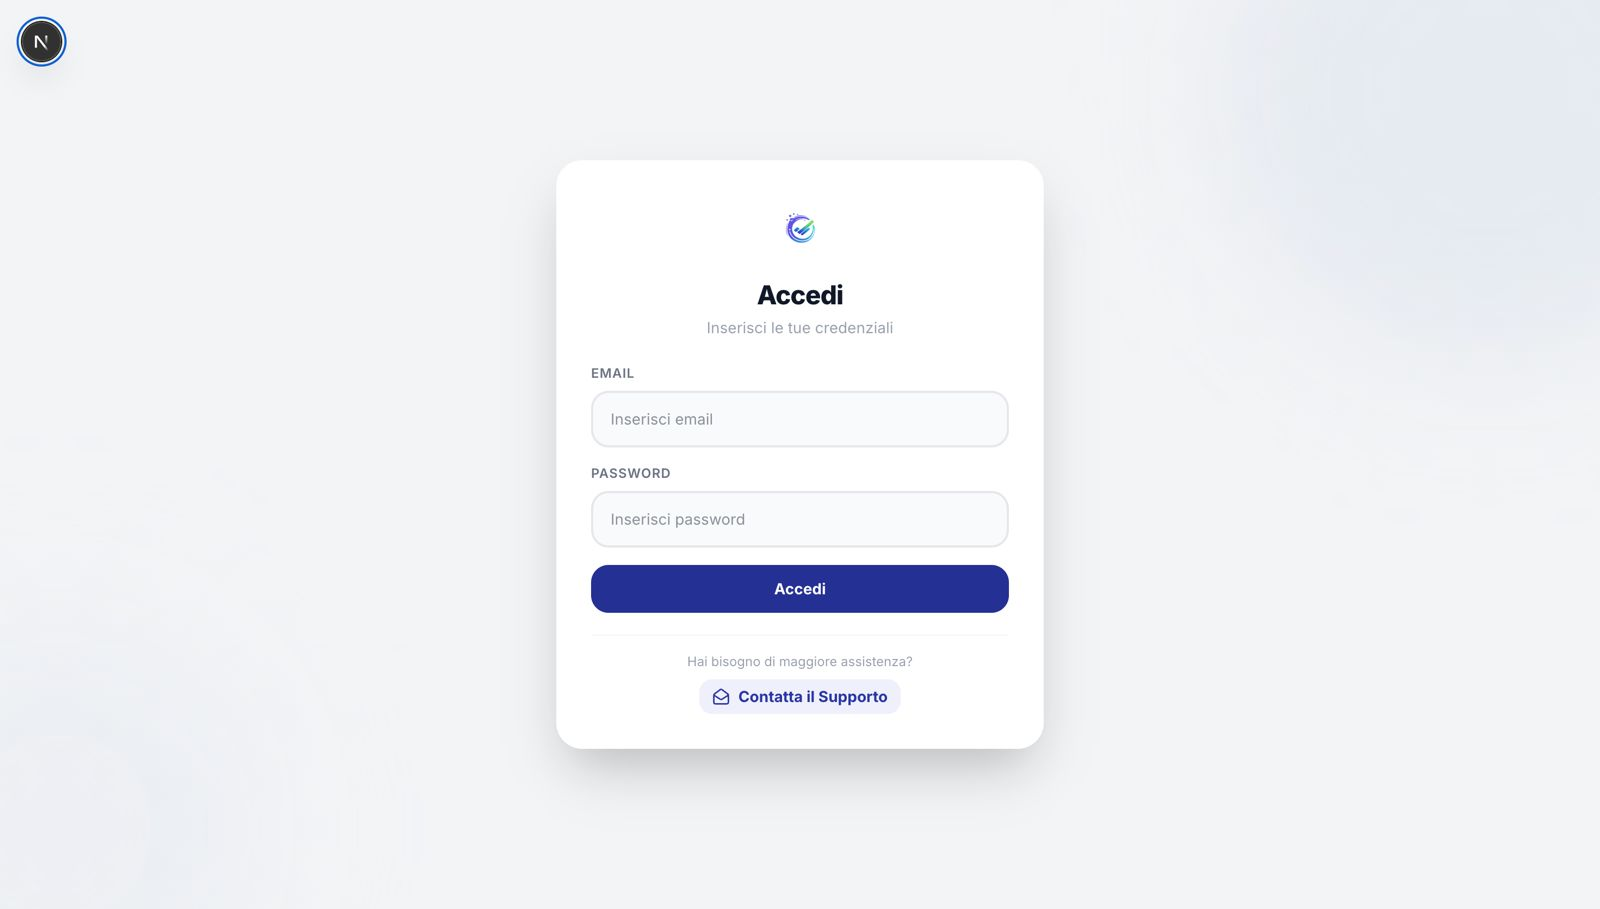
\includegraphics[width=0.7\textwidth]{Contenuti/immagini/login.jpeg}
    \caption{Schermata di login}
\end{figure}

All'apertura dell'applicazione viene visualizzata la schermata di autenticazione. L'utente inserisce le proprie credenziali (email e password) fornite dall'azienda nei campi dedicati e preme il pulsante \textbf{Accedi}.

Se le credenziali sono corrette e l'utente ha ruolo \textbf{Cliente}, viene immediatamente reindirizzato all'interfaccia principale di ordinazione. Se le credenziali appartengono a un utente con ruolo \textbf{Operatore}, viene effettuato un redirect automatico all'interfaccia di backoffice.

\`E inoltre possibile contattare il supporto direttamente dalla schermata di login tramite il pulsante \textbf{Contatta il Supporto}, che apre il client di posta predefinito con un template di richiesta assistenza precompilato.

\subsection{Logout}
Per disconnettersi dalla piattaforma, selezionare l'opzione \textbf{Logout} dal menu dell'area personale. La sessione viene invalidata e l'utente viene riportato alla schermata di login.


\newpage
\section{Panoramica delle funzionalit\`a}
Questa sezione fornisce una visione d'insieme delle funzionalit\`a offerte dalla piattaforma, suddivise per ruolo utente.

\subsection{Funzionalit\`a dell'Operatore}
\begin{description}[style=nextline, leftmargin=1.5cm]
    \item[\textbf{Dashboard ticket}] Visualizzazione tabellare di tutti i ticket aperti/in lavorazione, ordinati per tempo di attesa decrescente (i pi\`u urgenti in alto). Aggiornamento automatico in tempo reale.
    \item[\textbf{Gestione ticket}] Apertura di un pannello dedicato per ogni ticket con chat in tempo reale (SSE) e carrello del cliente modificabile. L'operatore pu\`o inviare messaggi, aggiungere/rimuovere/modificare articoli e inviare l'ordine per conto del cliente.
    \item[\textbf{Storico ordini globale}] Consultazione di tutti gli ordini di tutti i clienti con filtri avanzati per ID ordine, codice cliente, ragione sociale e intervallo date. Ordinamento multicolonna. Esportazione in formato JSON e CSV.
    \item[\textbf{Export batch}] Esportazione automatica degli ordini in formato CSV al login dell'operatore, salvati nella cartella configurata.
    \item[\textbf{Configurazione export}] Impostazione della cartella di salvataggio per i file di export ordini.
    \item[\textbf{Area personale}] Consultazione del proprio profilo e cambio password.
\end{description}

Per le funzionalit\`a riservate al Cliente si rimanda al \textit{Manuale Cliente}.


\newpage
\section{Istruzioni d'uso -- Operatore}

L'interfaccia Operatore \`e accessibile esclusivamente agli utenti con ruolo \texttt{admin}. Al login, se le credenziali appartengono a un operatore, viene effettuato un redirect automatico da \texttt{/} a \texttt{/operatore}.

L'interfaccia presenta un layout desktop con barra di navigazione laterale contenente tre sezioni: \textbf{Ticket Aperti}, \textbf{Storico Ordini}, \textbf{Profilo}. In alto a sinistra \`e visibile il nome dell'operatore; in alto a destra il pulsante di logout.

All'accesso, se \`e configurata una cartella di export, viene eseguito automaticamente un export batch degli ultimi ordini (fino a 50) e viene mostrata una notifica toast con il risultato.

\subsection{Dashboard e gestione ticket}

\begin{figure}[H]
    \centering
    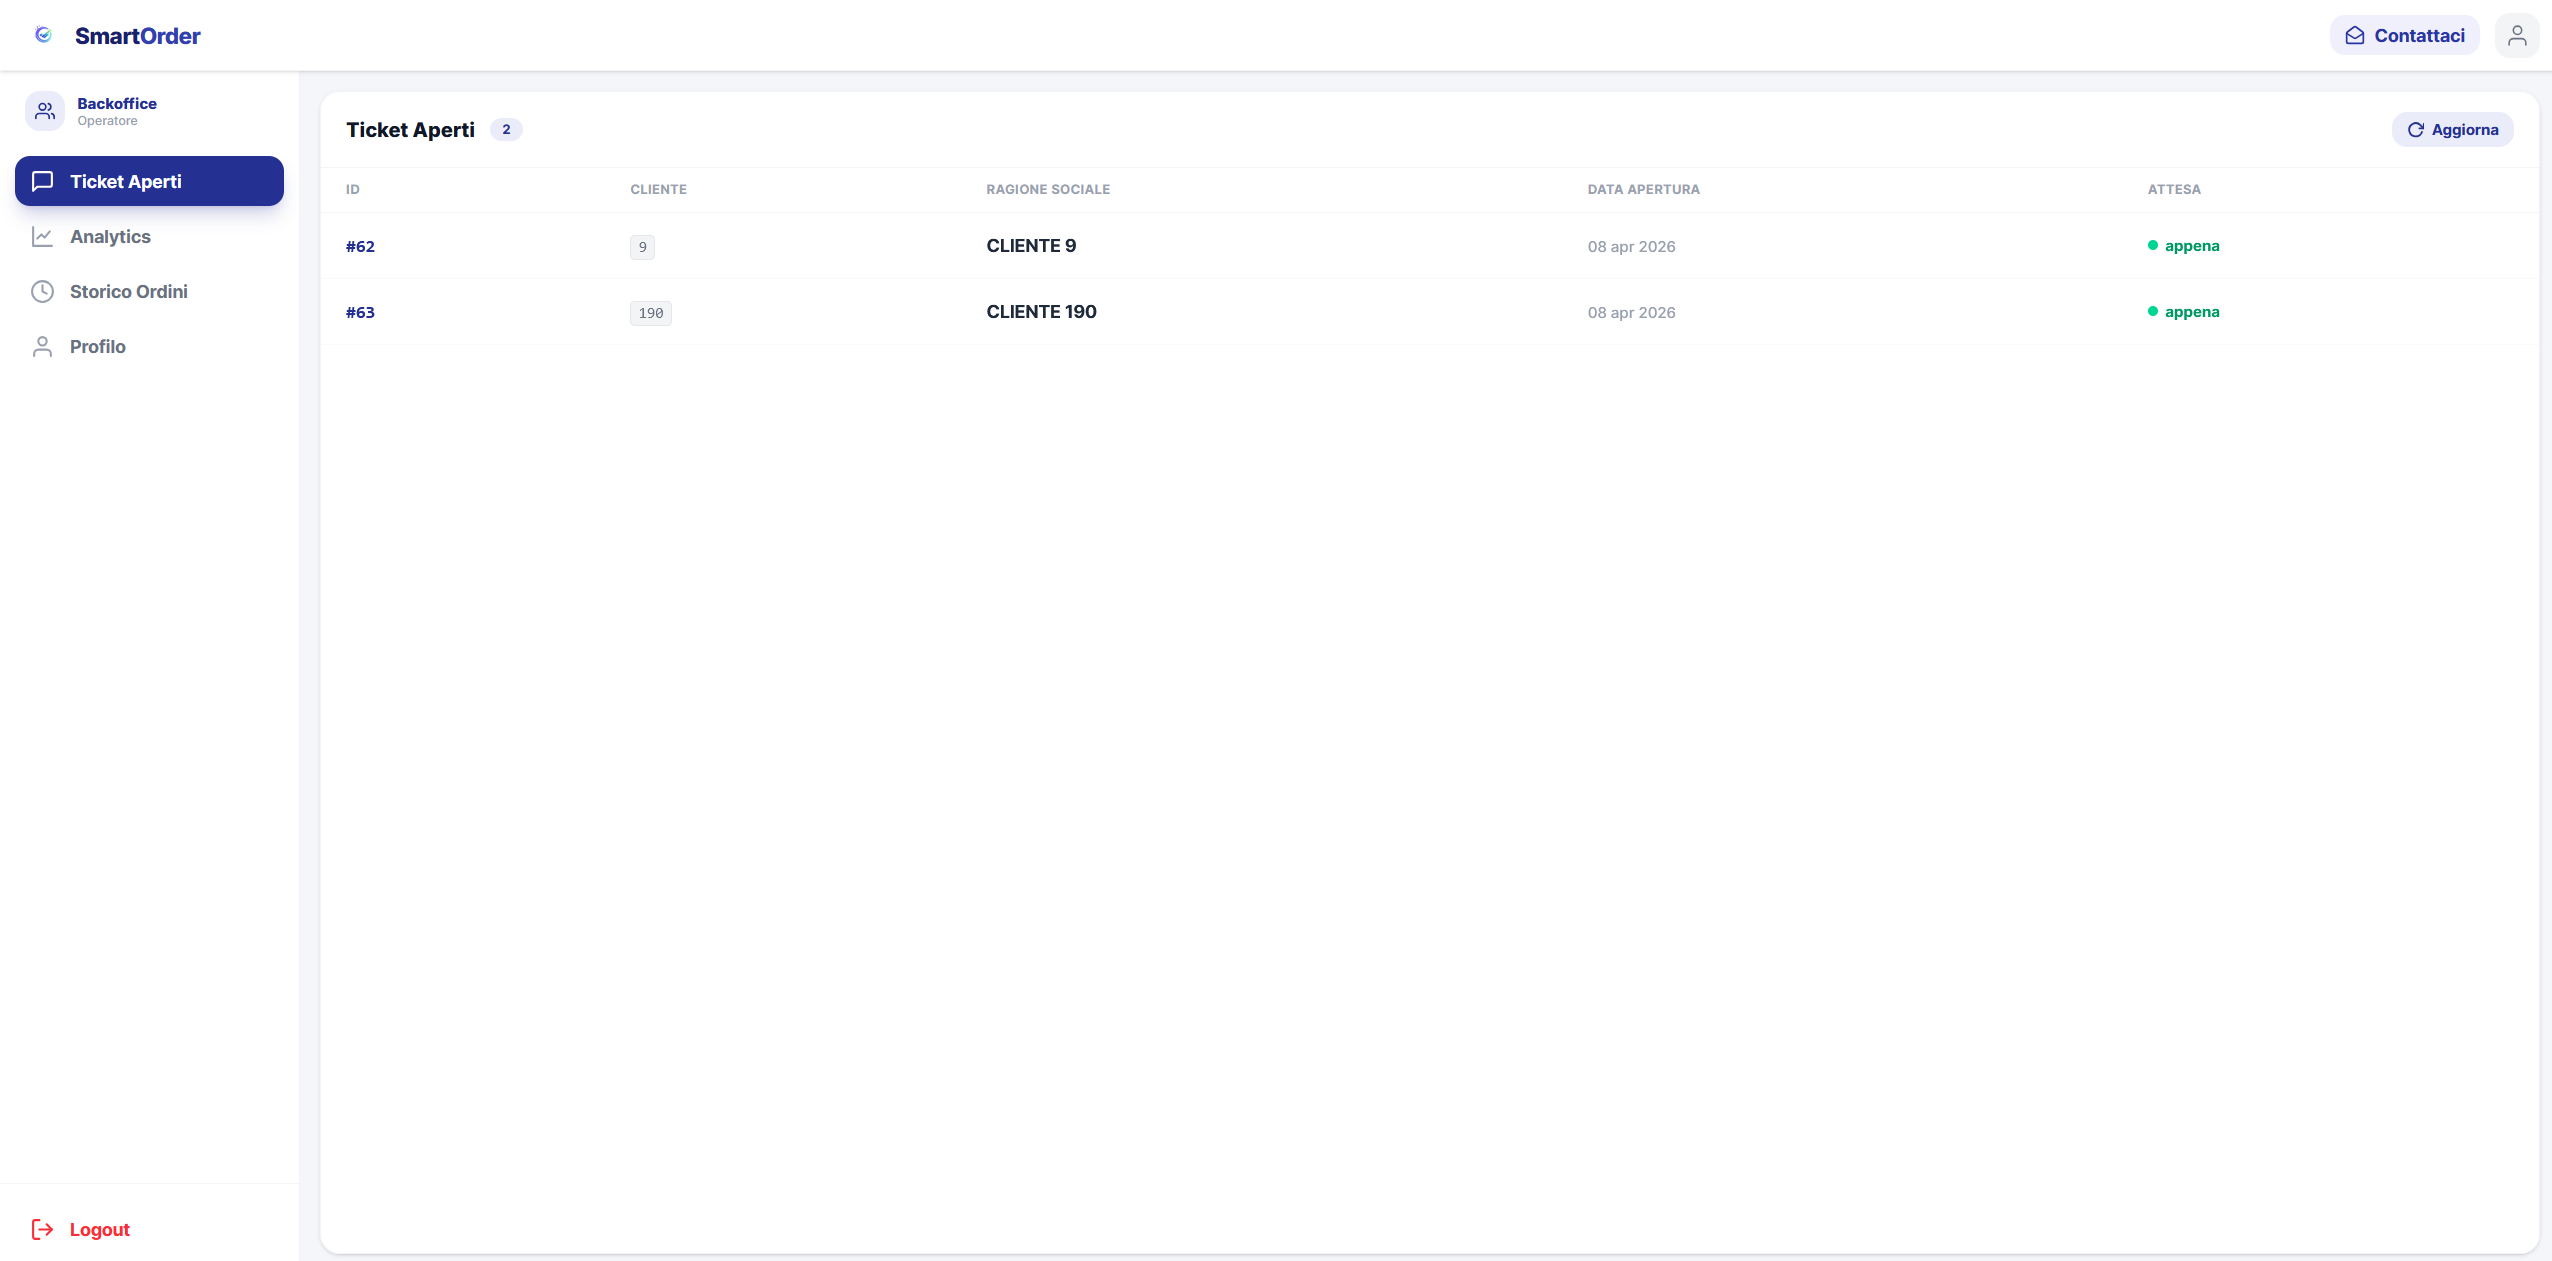
\includegraphics[width=0.7\textwidth]{Contenuti/immagini/lista ticket.png}
    \caption{Lista ticket aperti}
\end{figure}

La sezione \textbf{Ticket Aperti} \`e la vista predefinita dell'interfaccia operatore.

\subsubsection{Lista ticket}
\begin{enumerate}
    \item \textbf{Visualizzazione}: La tabella mostra tutti i ticket aperti e in lavorazione, ordinati per tempo di attesa decrescente (i pi\`u urgenti in cima). Ogni riga contiene: ID ticket, codice cliente (badge), ragione sociale, data di apertura e tempo di attesa.
    \item \textbf{Indicatore di gravit\`a}: Il tempo di attesa \`e colorato: rosso pulsante ($> 30$ minuti, urgente), ambra ($10$--$30$ minuti), verde ($< 10$ minuti).
    \item \textbf{Stato ticket}: Se un ticket \`e \texttt{In carico} (un operatore lo sta gi\`a gestendo), compare un badge ambra sulla riga.
    \item \textbf{Aggiorna}: Cliccare su \texttt{Aggiorna} in alto a destra per ricaricare la lista. L'elenco si aggiorna automaticamente anche in tempo reale tramite SSE.
    \item \textbf{Apertura ticket}: Cliccare su una riga qualsiasi per aprire il pannello di gestione del ticket.
\end{enumerate}

\subsubsection{Pannello di gestione ticket}

\begin{figure}[H]
    \centering
    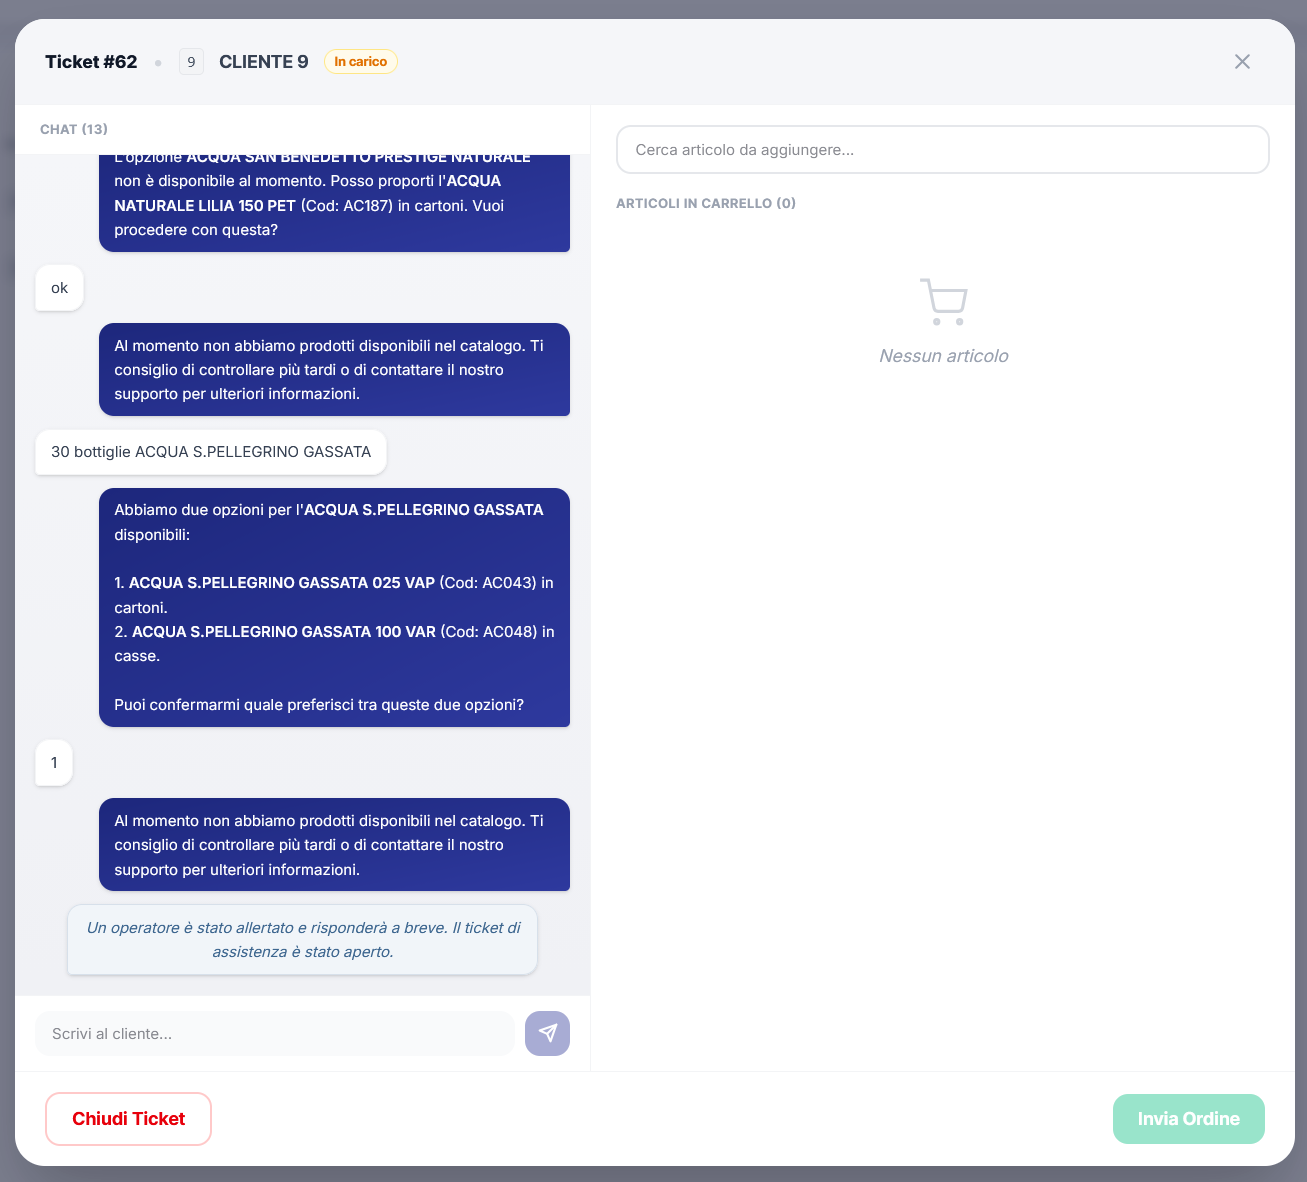
\includegraphics[width=0.7\textwidth]{Contenuti/immagini/ticket.png}
    \caption{Finestra di gestione ticket}
\end{figure}

Aprendo un ticket si accede a un modale a schermo intero suddiviso in tre aree:

\textbf{Header}: mostra l'ID ticket, il codice cliente, la ragione sociale e un badge di stato (Aperto o In carico). \`E presente il pulsante di chiusura (X).

\textbf{Area centrale sinistra (45\%)} -- \textbf{Chat}:
\begin{itemize}
    \item Elenco dei messaggi scambiati con il cliente (sia via IA che direttamente con l'operatore).
    \item I messaggi di sistema sono visualizzati in grigio corsivo centrato (ad esempio per segnalare che il ticket \`e stato aperto/assegnato).
    \item Vengono segnati i feedback inviati dai clienti
    \item Campo di input in basso per inviare messaggi di testo al cliente.
    \item I nuovi messaggi arrivano in tempo reale tramite SSE.
\end{itemize}

\textbf{Area centrale destra (55\%)} -- \textbf{Carrello Cliente}:
\begin{itemize}
    \item Campo di ricerca prodotti con autocomplete per aggiungere articoli al carrello del cliente.
    \item Elenco degli articoli attualmente nel carrello con possibilit\`a di modificarne le quantit\`a (pulsanti \texttt{+} e \texttt{-}) e rimuoverli (icona cestino).
    \item Badge \texttt{AI} e anello di confidenza per articoli aggiunti dall'IA.
    \item Il carrello si sincronizza in tempo reale sia con le azioni dell'operatore che con quelle del cliente.
\end{itemize}

\textbf{Area inferiore (footer)} -- \textbf{Azioni}:
\begin{itemize}
    \item \texttt{Chiudi Ticket}: Chiude il ticket definitivamente. Non viene inviato alcun ordine.
    \item \texttt{Invia Ordine}: Compila e invia l'ordine per conto del cliente usando il contenuto corrente del carrello, poi chiude automaticamente il ticket.
\end{itemize}

\subsection{Storico ordini (Operatore)}

\begin{figure}[H]
    \centering
    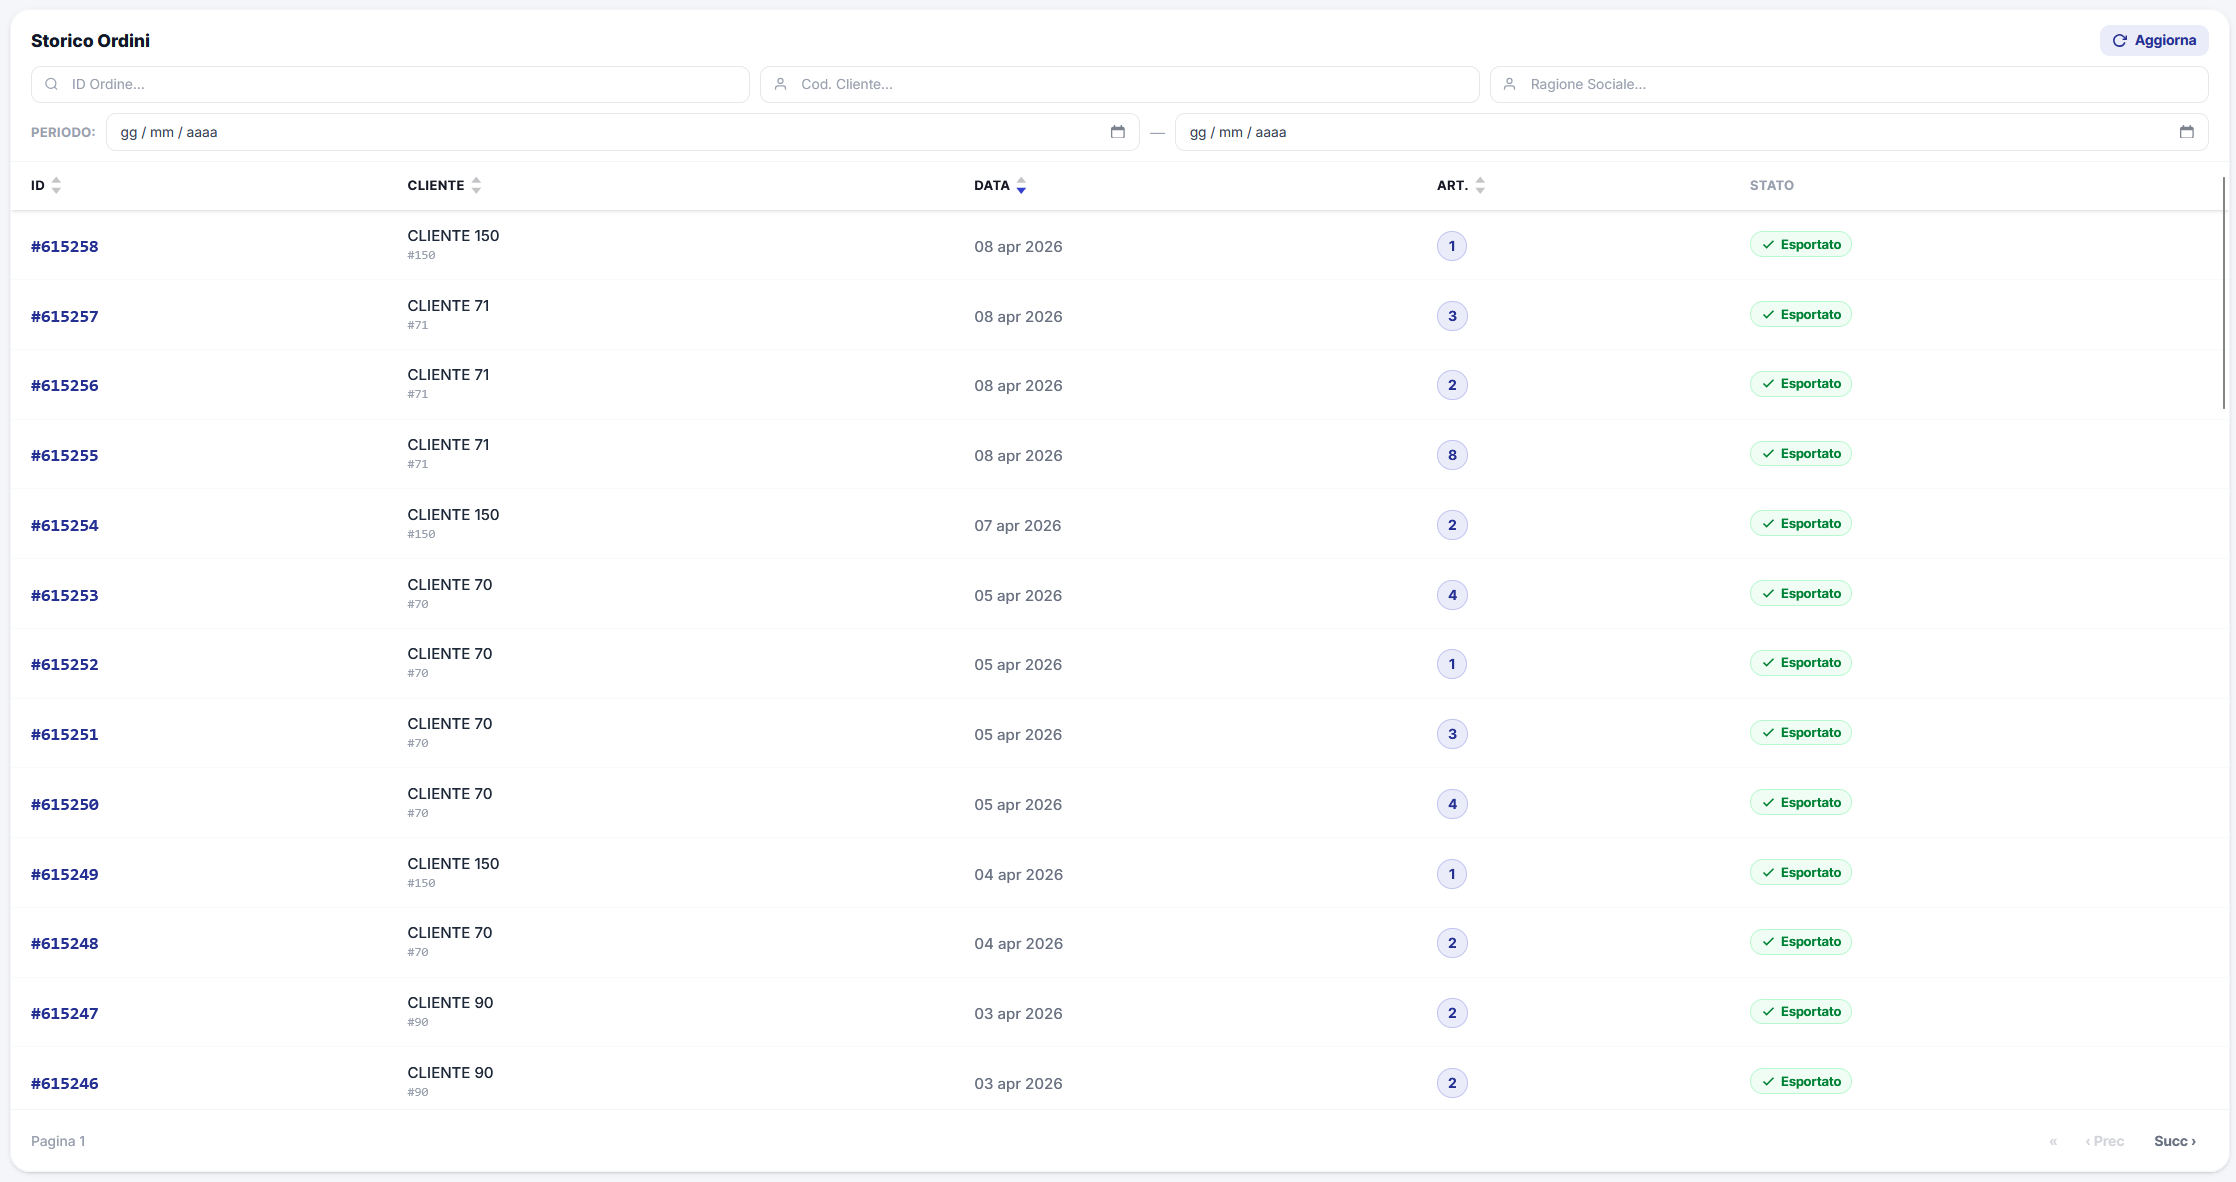
\includegraphics[width=0.7\textwidth]{Contenuti/immagini/storico operatore.png}
    \caption{Storico degli ordini}
\end{figure}

La sezione \textbf{Storico Ordini} consente la consultazione di tutti gli ordini di tutti i clienti.

\begin{enumerate}
    \item \textbf{Lista ordini}: Tabella con ordinamento multicolonna. Ogni riga mostra: ID ordine (cliccabile), ragione sociale cliente, data, numero di articoli e stato export.
    \item \textbf{Filtri avanzati}:
    \begin{itemize}
        \item Campo di ricerca per ID ordine.
        \item Campo per codice cliente.
        \item Campo per ragione sociale (ricerca debounced).
        \item Filtro per intervallo date (da -- a).
        \item Ordinamento per qualsiasi colonna (ID, cliente, data, articoli) con frecce di direzione.
    \end{itemize}
    \item \textbf{Pulsante X}: Cancella tutti i filtri attivi.
    \begin{figure}[H]
        \centering
        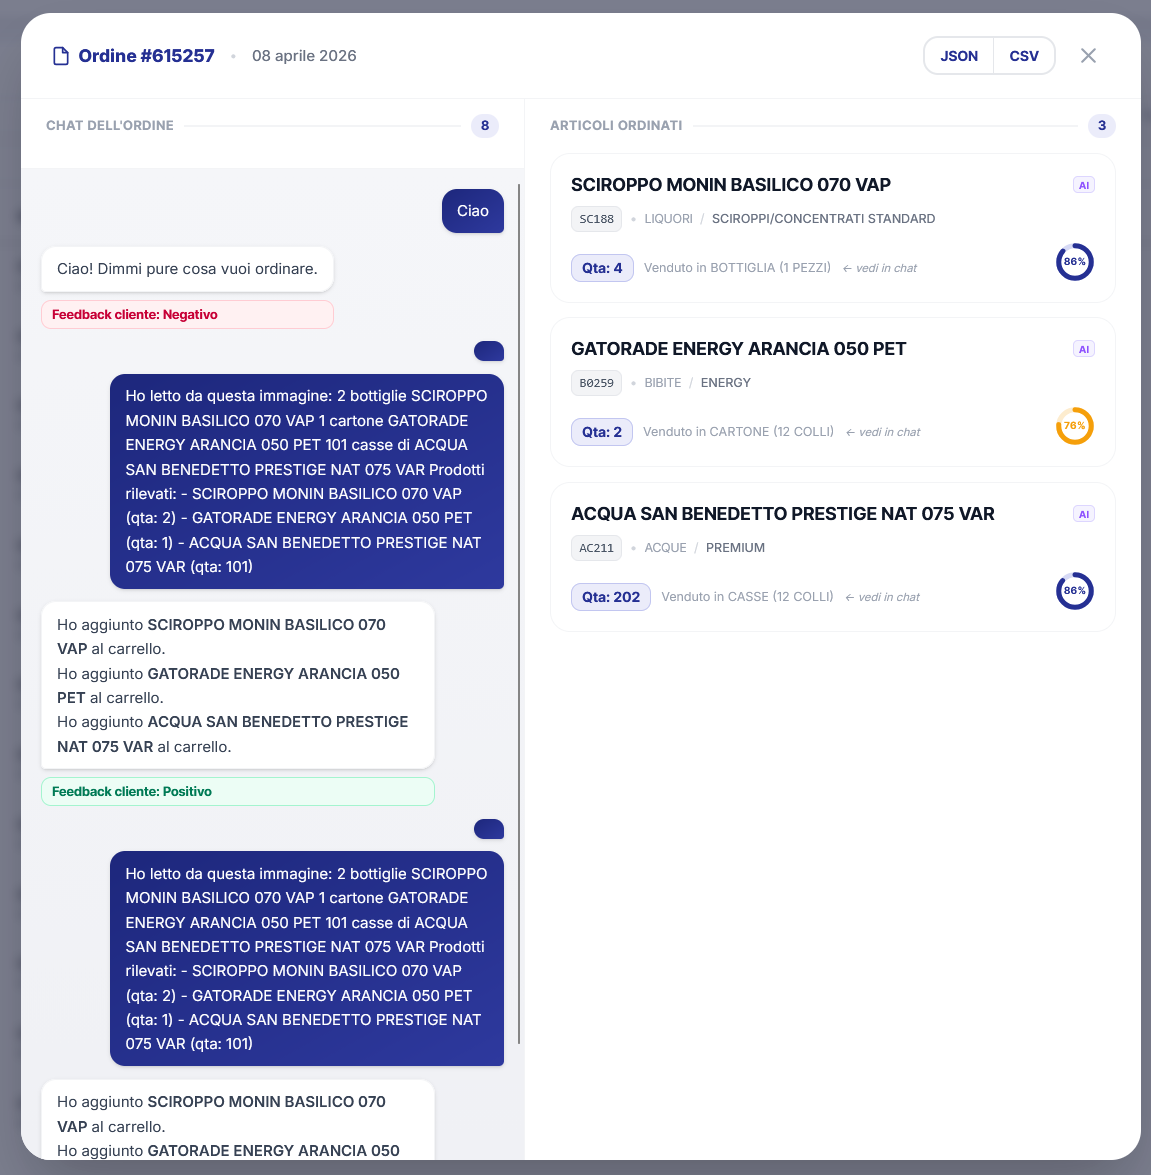
\includegraphics[width=0.7\textwidth]{Contenuti/immagini/dettagli ordine operatore.png}
        \caption{Dettagli ordine}
    \end{figure}
    \item \textbf{Dettaglio ordine}: Cliccando su una riga si apre un modale di dettaglio con:
    \begin{itemize}
        \item A sinistra: chat completa dell'ordine (se disponibile).
        \item A destra: elenco articoli ordinati con codice, descrizione, linea/famiglia, quantit\`a ordinata, unit\`a di misura e confidenza IA. Cliccando su un articolo con messaggio collegato si scrolla alla chat evidenziando il messaggio.
    \end{itemize}
    \item \textbf{Export}: Nel dettaglio ordine sono presenti i pulsanti \texttt{JSON} e \texttt{CSV} per esportare l'ordine singolarmente. Il file viene salvato nella cartella configurata nelle variabili d'ambiente.
    \item \textbf{Export batch}: Al login, se la cartella di export \`e configurata, viene eseguito automaticamente un export batch degli ordini non ancora esportati (fino a 50). Il risultato viene notificato tramite toast.
    \item \textbf{Stato export}: Nella lista ordini, la colonna \texttt{Stato} mostra un badge verde \texttt{Esportato} se l'ordine \`e gi\`a stato esportato, oppure un trattino se non ancora esportato.
\end{enumerate}

\subsection{Analytics}

\begin{figure}[H]
        \centering
        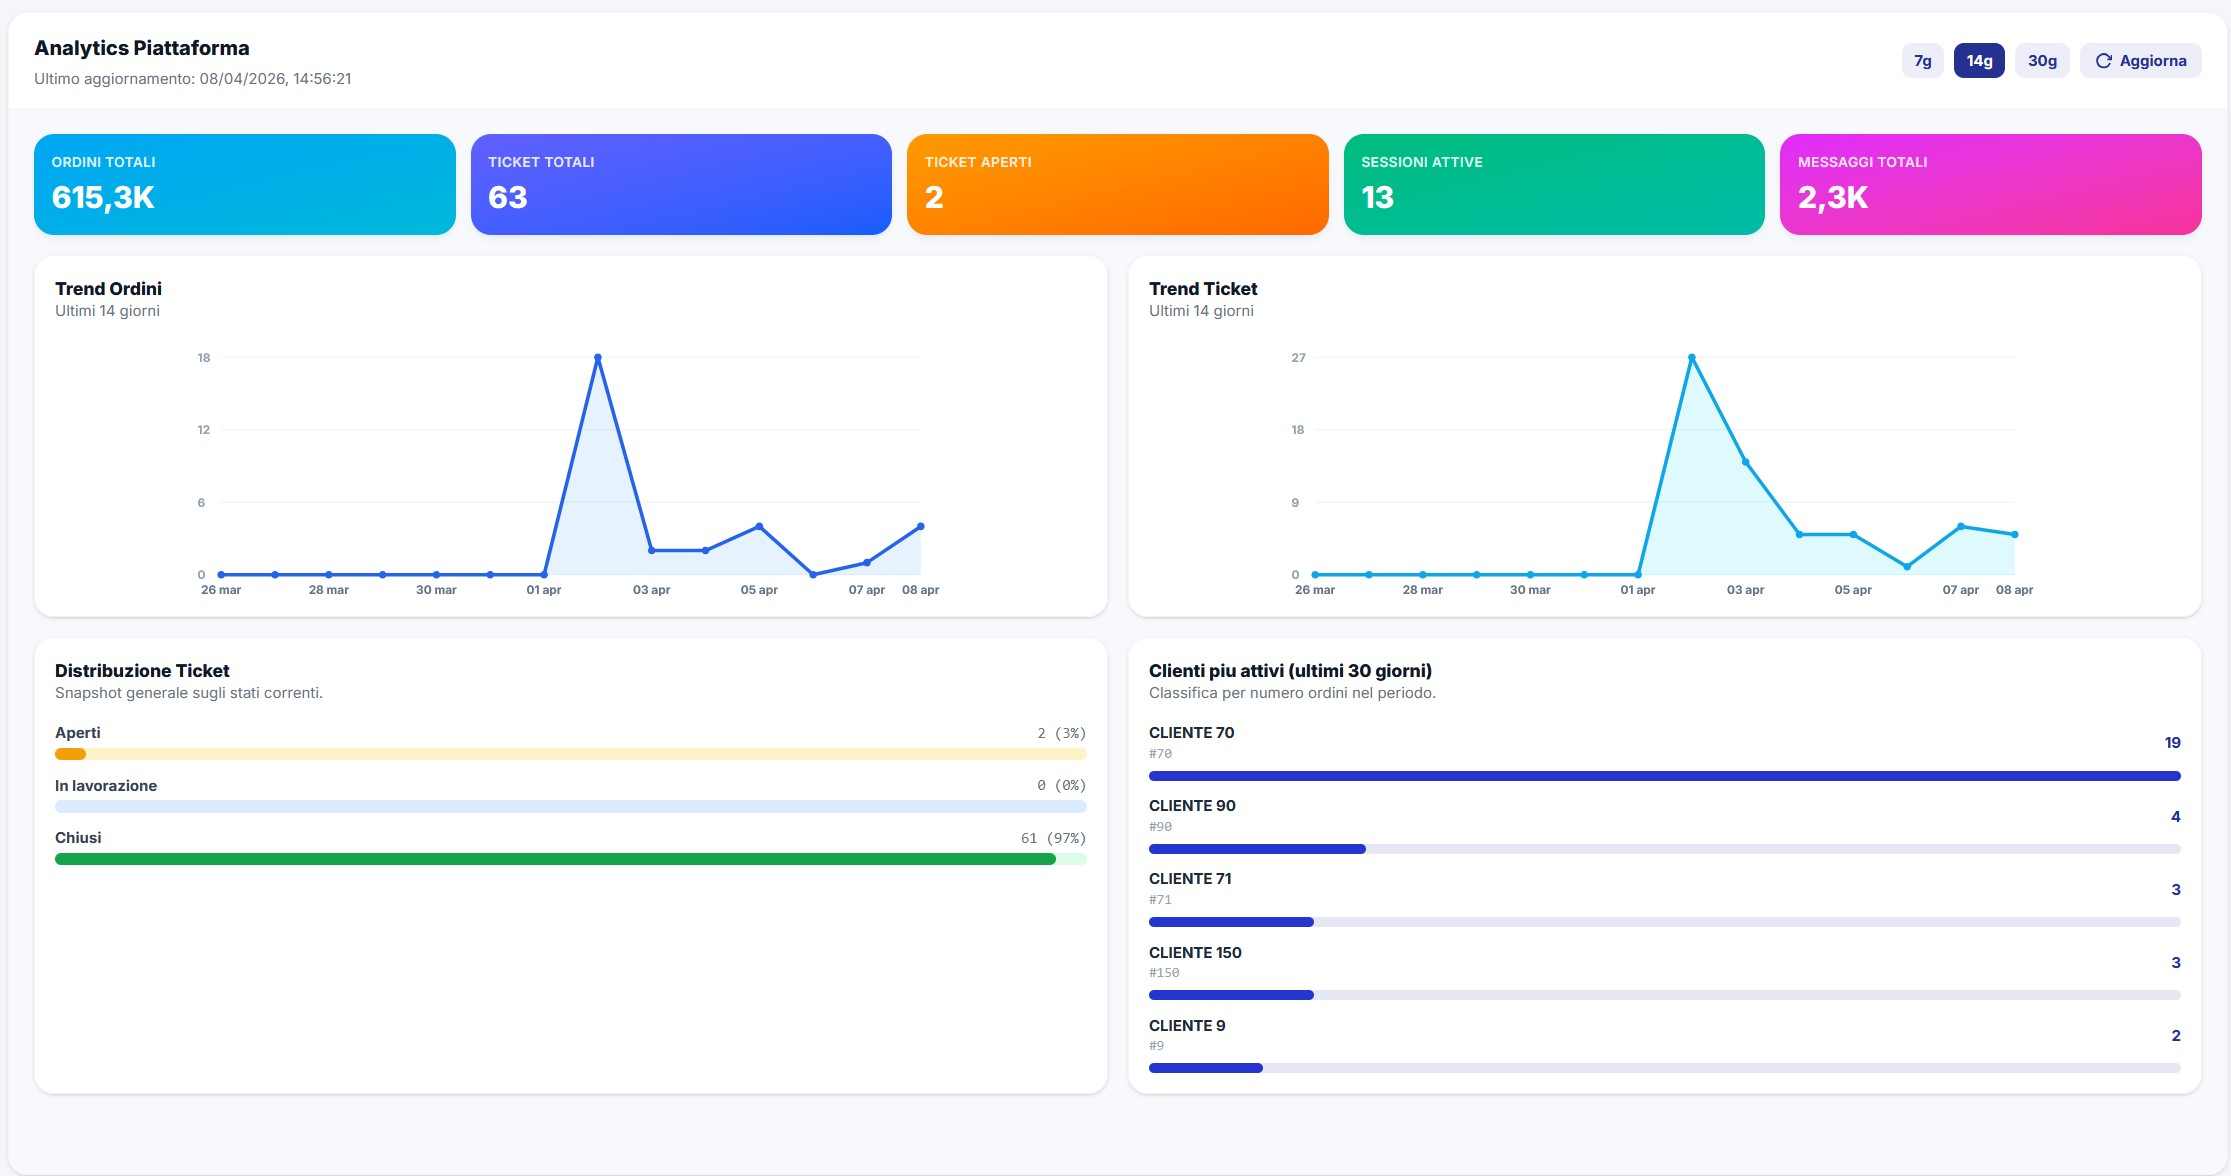
\includegraphics[width=0.8\textwidth]{Contenuti/immagini/analytics.jpeg}
        \caption{Statistiche del sistema}
    \end{figure}

È disponibile una schermata \textbf{analytics} che permette di vedere:
\begin{enumerate}
    \item Gli ordini totali effettuati dal sistema.
    \item I ticket totali.
    \item I ticket attualmente aperti
    \item Le sessioni attive al momento
    \item Il numero di messaggi inviati al sistema
    \item Il trend di ordini e tricket nel periodo scelto (7, 14 o 30 giorni)
    \item Un riepilogo dei ticket aperti, in lavorazione e chiusi
    \item L'elenco dei clienti più attivi
\end{enumerate}

\subsection{Area personale (Operatore)}

\begin{figure}[H]
    \centering
    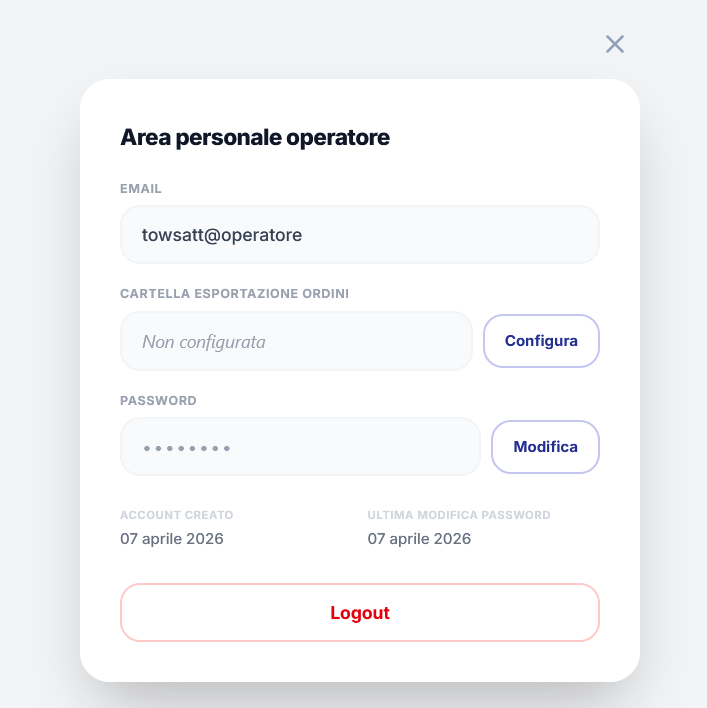
\includegraphics[width=0.7\textwidth]{Contenuti/immagini/area personale operatore.png}
    \caption{Area personale dell'operatore}
\end{figure}
\begin{figure}[H]
    \centering
    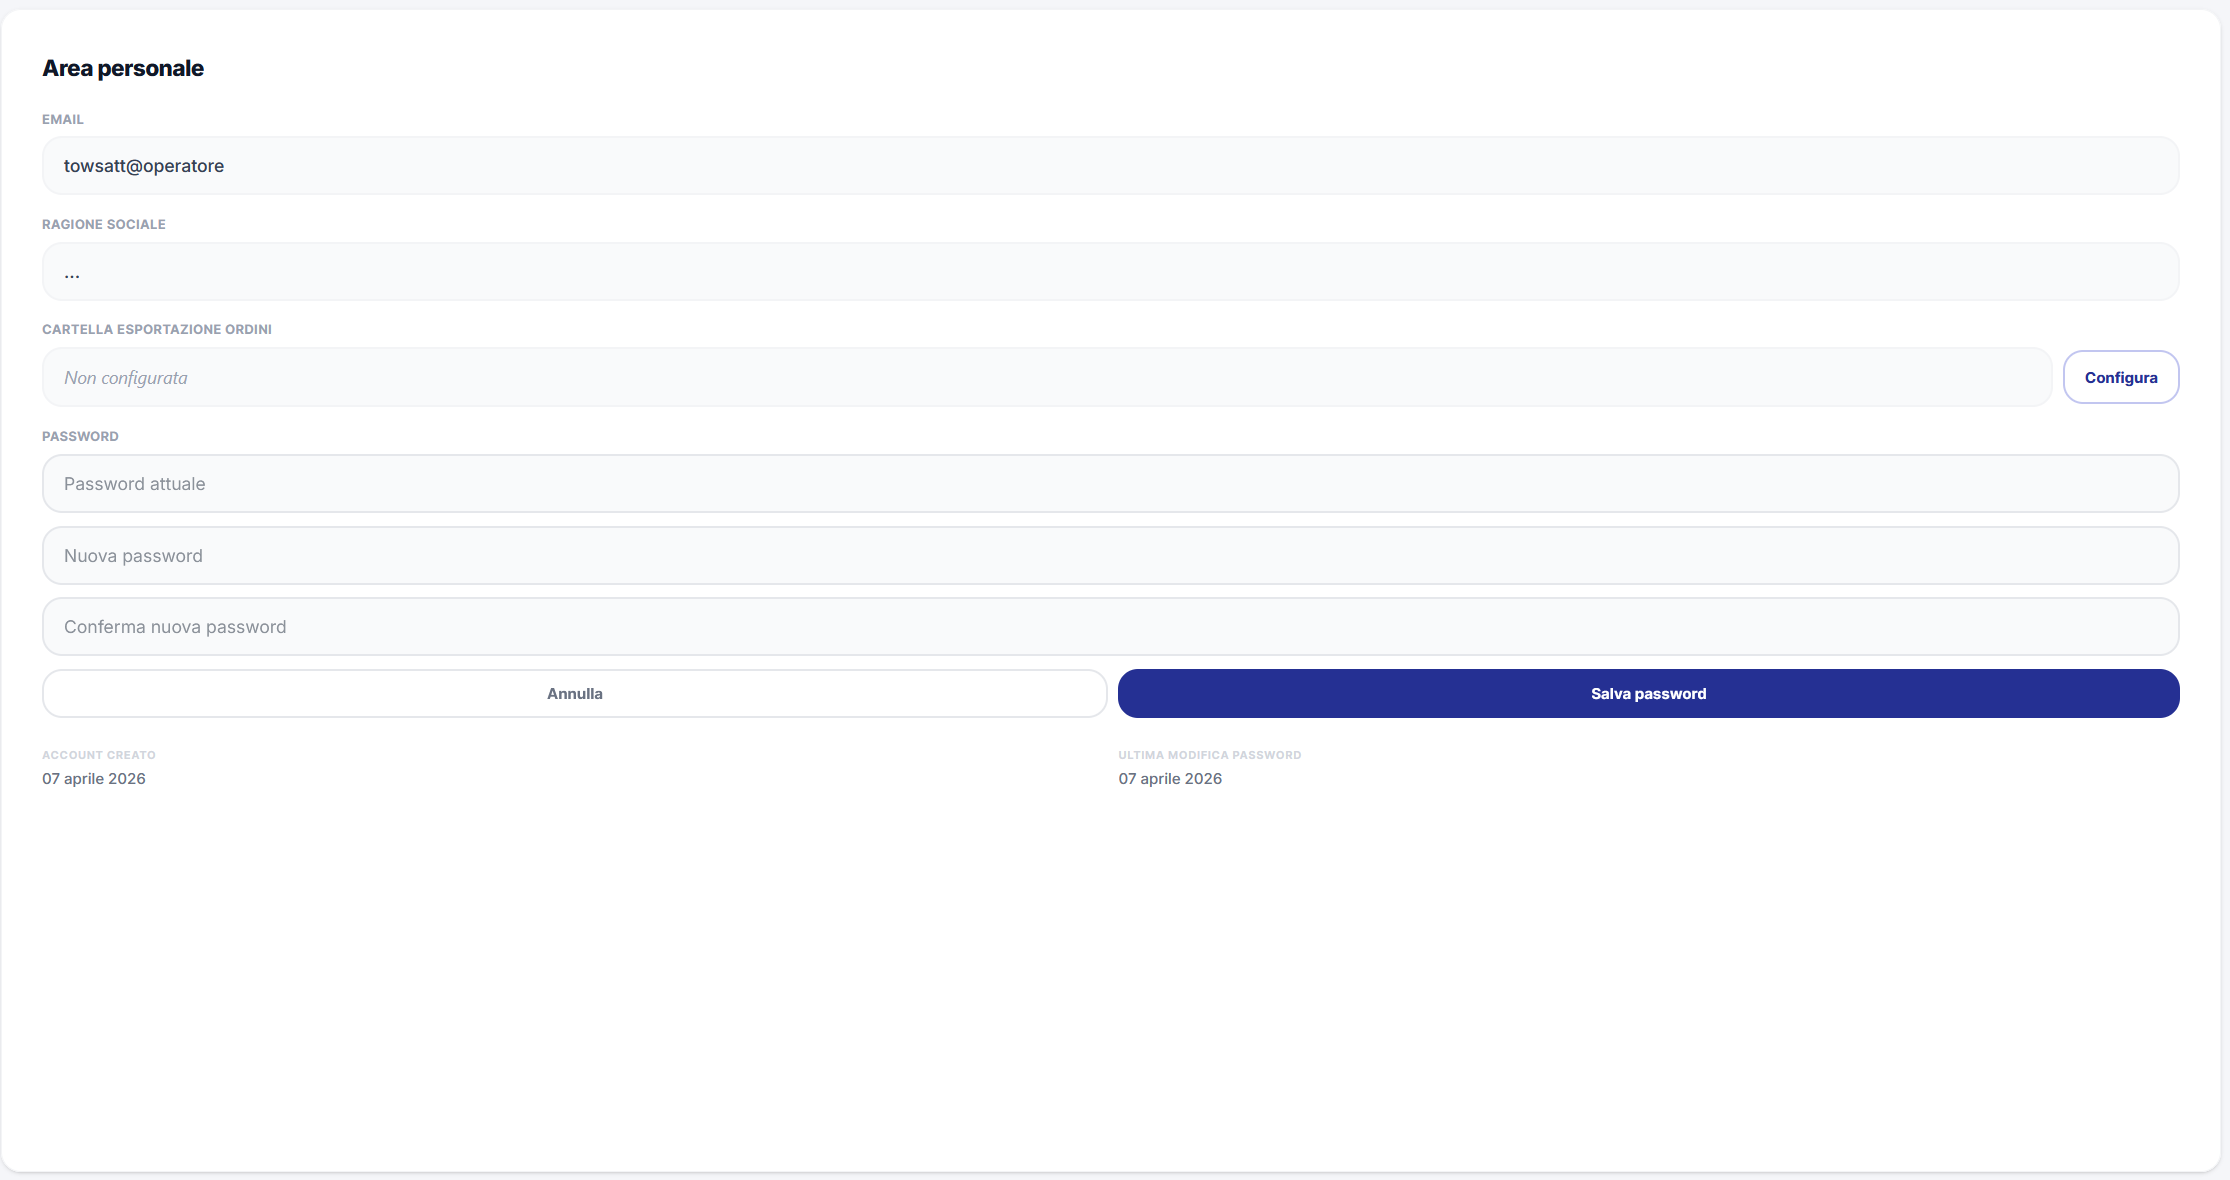
\includegraphics[width=0.7\textwidth]{Contenuti/immagini/cambio password operatore.png}
    \caption{Cambio password dell'account}
\end{figure}

Per accedere alle impostazioni del profilo:

\begin{enumerate}
    \item \textbf{Apertura}: Selezionare la sezione \texttt{Profilo} nella barra di navigazione laterale.
    \item \textbf{Dati}: Vengono mostrate email e ragione sociale dell'account operatore, oltre alle date di creazione account e ultima modifica password.
    \item \textbf{Cartella di export}: Sezione dedicata (presente solo per admin) per configurare il percorso della cartella in cui verranno salvati i file CSV/JSON degli ordini esportati. Cliccare su \texttt{Configura} o \texttt{Modifica} per impostare il path assoluto (es. \texttt{/Users/davide/ordini}), poi \texttt{Salva}.
    \item \textbf{Cambio password}: Cliccare su \texttt{Modifica} nella sezione password, inserire la password attuale, la nuova (minimo 6 caratteri) e la conferma, poi \texttt{Salva password}.
    \item \textbf{Logout}: Cliccare su \texttt{Logout} in fondo alla schermata.
\end{enumerate}


\newpage
Di seguito sono elencati i principali messaggi di errore che l'utente potrebbe incontrare durante l'utilizzo della piattaforma, con le relative soluzioni suggerite.

\begin{longtable}{|p{4cm}|p{4cm}|p{5.5cm}|}
    \caption{Tabella messaggi di errore e soluzioni.}
    \label{tab:errori} \\
    \hline
    \rowcolor{gray!10} \textbf{Messaggio / Situazione} & \textbf{Causa probabile} & \textbf{Soluzione} \\
    \hline
    \endfirsthead
    \hline
    \rowcolor{gray!10} \textbf{Messaggio / Situazione} & \textbf{Causa probabile} & \textbf{Soluzione} \\
    \hline
    \endhead
    \hline
    \endfoot

    \textit{``Errore di rete durante il login''} & Credenziali non corrette o server non raggiungibile & Verificare di aver inserito email e password corretti. Controllare la connessione a internet. \\
    \hline
    \textit{``Impossibile accedere al microfono''} & Browser non ha (o ha negato) il permesso di usare il microfono & Concedere il permesso del microfono nelle impostazioni del browser. Ricaricare la pagina. \\
    \hline
    \textit{``Non ho capito nulla dall'audio. Puoi ripetere o scrivere?''} & Audio troppo basso, rumore di fondo eccessivo o vocabolario non riconosciuto & Ripetere la frase in modo pi\`u chiaro, avvicinarsi al microfono, diminuire i rumori ambientali. In alternativa, digitare il testo. \\
    \hline
    \textit{``Servizio chat non disponibile. Verifica che il servizio Python sia attivo sulla porta 8000.''} & Il backend FastAPI non \`e in esecuzione & Avviare il backend con \texttt{python main.py} nella directory \texttt{backend}. Verificare che stia ascoltando sulla porta corretta. \\
    \hline
    Articolo evidenziato in rosso nel carrello: \texttt{Articolo non pi\`u disponibile} & Il prodotto non \`e pi\`u disponibile nel catalogo al momento dell'invio dell'ordine & Rimuovere l'articolo dal carrello prima di inviare nuovamente l'ordine. \\
    \hline
    Articolo non aggiunto al carrello (``Alcuni prodotti non risultano al momento disponibili'') & Il codice articolo richiesto non corrisponde a nessun prodotto nel catalogo dell'utente & Provare a descrivere il prodotto con altre parole chiave, oppure cercarlo manualmente nel catalogo. \\
    \hline
    \textit{``Errore invio ordine''} con codice articolo specifico & Il backend ha rifiutato l'articolo per vincoli di catalogo o autorizzazione & Rimuovere l'articolo indicato dall'errore e riprovare. Se il problema persiste, contattare il supporto. \\
    \hline
    \textit{``Articolo bloccato: [stato]''} & L'articolo ha uno stato che ne impedisce l'aggiunta (sospeso, su autorizzazione, non disponibile) & Non \`e possibile aggiungere questo articolo. Provare con un'alternativa o contattare l'assistenza. \\
    \hline
    La lista ticket non si aggiorna & Connessione SSE interrotta & Cliccare su \texttt{Aggiorna} per ricaricare manualmente. Verificare la connessione a internet. \\
    \hline
    \textit{``Errore di rete''} in qualsiasi operazione & Temporanea indisponibilit\`a del server o della connessione & Attendere qualche secondo e riprovare. Se il problema persiste, ricaricare la pagina. \\
    \hline
    \textit{``Le due password non corrispondono''} & Errore di digitazione nel campo conferma password & Verificare che i campi \texttt{Nuova password} e \texttt{Conferma password} siano identici. \\
    \hline
    \textit{``La nuova password deve avere almeno 6 caratteri''} & Password troppo corta & Scegliere una nuova password di almeno 6 caratteri. \\
    \hline
    \textit{``Password attuale''} non accettata & Password attuale errata & Verificare di star inserendo la password corrente correttamente. \\
    \hline
    Export batch fallito (toast: ``ordini esportati, X falliti'') & Errore nella scrittura dei file nella cartella export configurata & Verificare che la cartella di export esista e che l'utente abbia i permessi di scrittura su di essa. Controllare il path configurato nel profilo operatore. \\
    \hline
    \end{longtable}


\newpage
Per segnalazioni, richieste di assistenza o feedback relativi al presente manuale o al sistema SmartOrder, \`e possibile contattare il gruppo NightPRO all'indirizzo:

\begin{center}
    \large \leavevmode\href{swe.nightpro@gmail.com}{swe.nightpro@gmail.com}
\end{center}


\end{document}
